

The Object Management Group's Interface Definition Language (IDL) is a 
subset of the \CPP \space programming language with additional keywords 
added for distributed concepts.  IDL does not include any algorithmic 
structures or variables.  While IDL syntax is similar to \CPP , the 
semantics of the languages are very different.  
\cite{siegel}  IDL is the strongly typed language used to 
provide a very strict definition of CORBA objects.   This strict definition 
is used to {\em{map}} IDL to a programming language so a programmer 
can implement and communicate with CORBA objects.  
IDL defines basic, constructed, and template types.  \cite{siegel}
The basic IDL types are listed in figure \ref{BasicIDLTypes}.  
In addition to these basic types, IDL offers structures and arrays.
In order to ensure interoperability, OMG's official language mappings 
map every IDL type to something in every mapped language.  \cite{siegel}
For the most complete and current information related to IDL, please 
refer to OMG's Official Website: {\em{http://www.omg.org}}. The IDL grammar 
, according to the CORBA 2$.$4 specification, is included in the appendix. 

\begin{figure}
\begin{center}
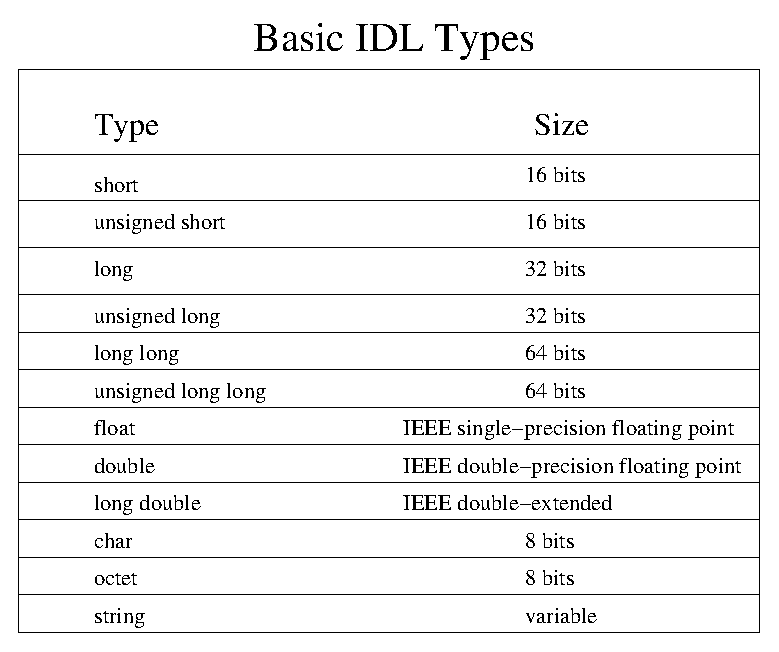
\psfig{file=Figures/BasicIDLTypes.eps}
\leavevmode
\caption{\em{The Basic IDL Types}.}
\label{BasicIDLTypes}
\end{center}
\end{figure}


